\documentclass[aspectratio=169]{beamer}
% \usepackage{listings}
\usepackage{hyperref}

\usepackage{minted}
\setminted{autogobble=true, linenos=false, fontsize=\scriptsize}
\usemintedstyle{friendly}

\usetheme{metropolis}

\title{How to recover from \texttt{chmod -x chmod}?}
\author{Felix Wittwer}
\date{ESE 2019}
\institute{NERD101 - TU Dresden}
\titlegraphic{\hfill
\includegraphics[height=1.25cm]{../logo}}

\begin{document}

\maketitle

\begin{frame}
    \centering
    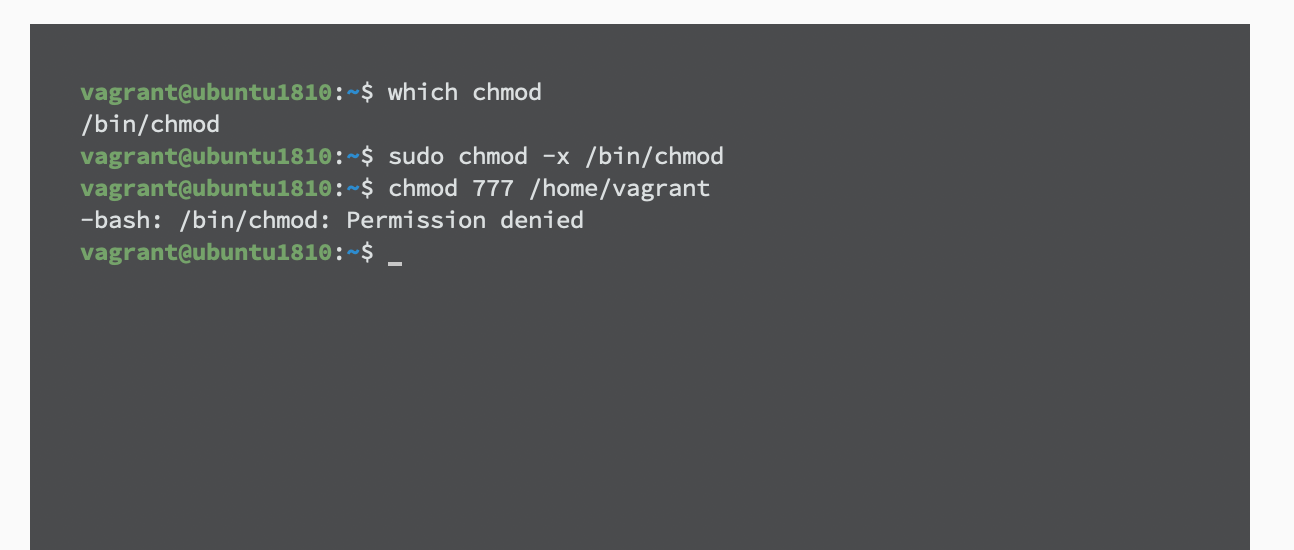
\includegraphics[width=.75\textwidth, keepaspectratio]{chmod.png}
    \pause

    The classic joke.

    But how does one recover from that? \uncover<3->{\emph{Without rebooting.}}
\end{frame}

\begin{frame}[fragile]{Using another programming language}
    \flushleft
    Most programming languages have their own implementation of \texttt{chmod}.
    \pause
    \vfill
    \begin{columns}[onlytextwidth]
        \begin{column}{.5\textwidth}
            C:
            \begin{minted}{c}
                #include <sys/types.h>
                #include <sys/stat.h>

                int main () {
                    chmod( "/bin/chmod", 0000755 );
                }
            \end{minted}
        \end{column}
        \begin{column}{.5\textwidth}
            \pause
            Python:
            \begin{minted}{python}
                import os
                os.chmod('/bin/chmod', 0755)
            \end{minted}
        \end{column}
    \end{columns}
\end{frame}

\begin{frame}[fragile]{Create another executable with \texttt{chmod}}
    Why write any new code at all?
    \pause
    \vfill
    \begin{columns}[onlytextwidth]
        \begin{column}{.5\textwidth}
            chmod.c
            \begin{minted}{c}
                int main () { }
            \end{minted}
        \end{column}
        \begin{column}{.5\textwidth}
            \pause
            \begin{minted}{text}
                $ gcc chmod.c
            \end{minted}
            \pause
            \begin{minted}{text}
                $ cat /bin/chmod > a.out
            \end{minted}
            \pause
            \begin{minted}{text}
                $ ./a.out +x /bin/chmod
            \end{minted}
        \end{column}
    \end{columns}
\end{frame}

\begin{frame}{Using GNU \texttt{tar}}
    \centering
    \texttt{tar} is a mighty tool!

    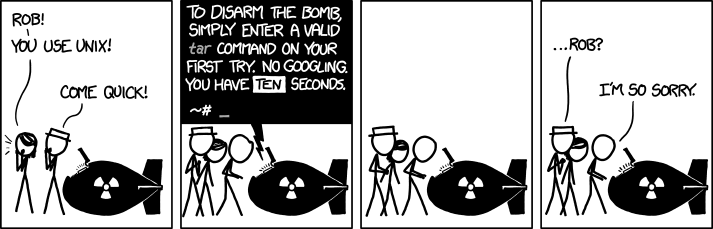
\includegraphics[width=.9\textwidth, keepaspectratio]{tar.png}
 \end{frame}

\begin{frame}[fragile]{Using GNU \texttt{tar}}
        \begin{itemize}
            \item Create an archive with specific permissions\\
                \pause \begin{minted}{text}
                    $ tar --mode 0755 -cf chmod.tar /bin/chmod
                    $ tar xvf chmod.tar
                \end{minted}
            \pause
            \item Or do the literally same thing without writing it to disk\\
                \pause \begin{minted}{text}
                    $ tar --mode 755 -cvf - /bin/chmod | tar xvf -
                \end{minted}
        \end{itemize}
\end{frame}

\begin{frame}[fragile]{With dynamic loaders}
    Use Linux' dynamic linker to load and run our broken binary.

    \begin{minted}{text}
        $ /bin/ld.so /bin/chmod +x chmod
    \end{minted}
\end{frame}

\begin{frame}[fragile]{Time travelling with \texttt{git}}
    Git can version software -- and modify attributes!
    \vfill

    \pause
    \begin{columns}[onlytextwidth]
        \begin{column}{.5\textwidth}
            Setup test environment:
        \end{column}
        \begin{column}{.5\textwidth}
            \begin{minted}{text}
                $ mkdir sandbox
                $ mv chmod sandbox/
                $ cd sandbox
            \end{minted}
        \end{column}
    \end{columns}

    \pause
    \begin{columns}[onlytextwidth]
        \begin{column}{.5\textwidth}
            Create an empty repository:
        \end{column}
        \begin{column}{.5\textwidth}
            \begin{minted}{text}
                $ git init
                $ git add chmod
                $ git commit -m '1985'
            \end{minted}
        \end{column}
    \end{columns}

    \pause
    \begin{columns}[onlytextwidth]
        \begin{column}{.5\textwidth}
            \alert{Time Travel Magic:}
        \end{column}
        \begin{column}{.5\textwidth}
            \begin{minted}{text}
                $ rm chmod
                $ git-update-index --chmod=+x chmod
                $ git checkout '1985'
            \end{minted}
        \end{column}
    \end{columns}
\end{frame}

\begin{frame}[fragile]{Fighting fire with fire}
    We can use emacs to fix this:

    \begin{minted}{lisp}
        Ctrl+x b > *scratch*
        (set-file-modes "/bin/chmod" (string-to-number "0755" 8))
        Ctrl+j
    \end{minted}
\end{frame}

\begin{frame}[fragile]{Using vim}
    The editor for every use case:

    \begin{minted}{text}
        $ vim -c "call setfperm('chmod', 'rwxrwxrwx') | quit"
    \end{minted}
\end{frame}

% https://unix.stackexchange.com/questions/295925/how-can-i-recover-from-a-chmod-x-chmod

\end{document}
